\documentclass[12pt, a4paper]{article}
\usepackage[a4paper, bindingoffset=0.2in, %
left=0.5in,right=0.5in,top=0.5in,bottom=0.5in,%
footskip=.25in]{geometry}
\usepackage{graphicx}
\usepackage{amssymb}
\usepackage{amsmath}
\usepackage{hyperref}
\usepackage{physics}

\title{PSet10 Report}
\author{Ali Abolhassanzadeh Mahani}

\begin{document}
	\maketitle
	I made a class \texttt{System} which consists of \texttt{Player} objects. The players play in the system and their utilities get updated.
	\section{Section 1}
	The plot for  Q over time is drawn in Fig~\ref{fig:Qs} for various values of beta.
	\begin{figure}[h!]
		\centering
		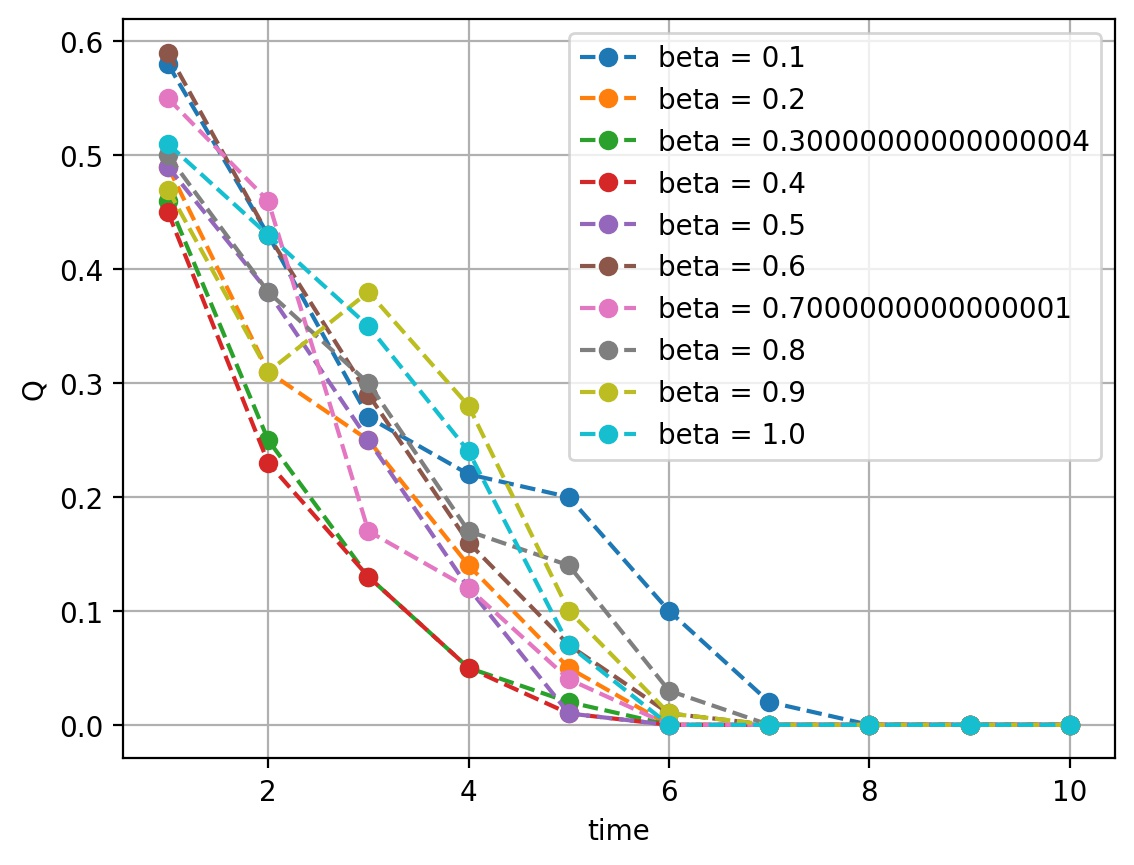
\includegraphics[width=.9\linewidth]{../results/Q_t_betas.jpg}
		\caption{As we can see, the equilibrium of the system is 0}
		\label{fig:Qs}
	\end{figure}
	
	\section{Section 2}
	Changing the equilibrium can be easily achieved by taking the transpose of the utility matrix. The results are in Fig~\ref{fig:Qs_inverse}.
	\begin{figure}[h!]
		\centering
		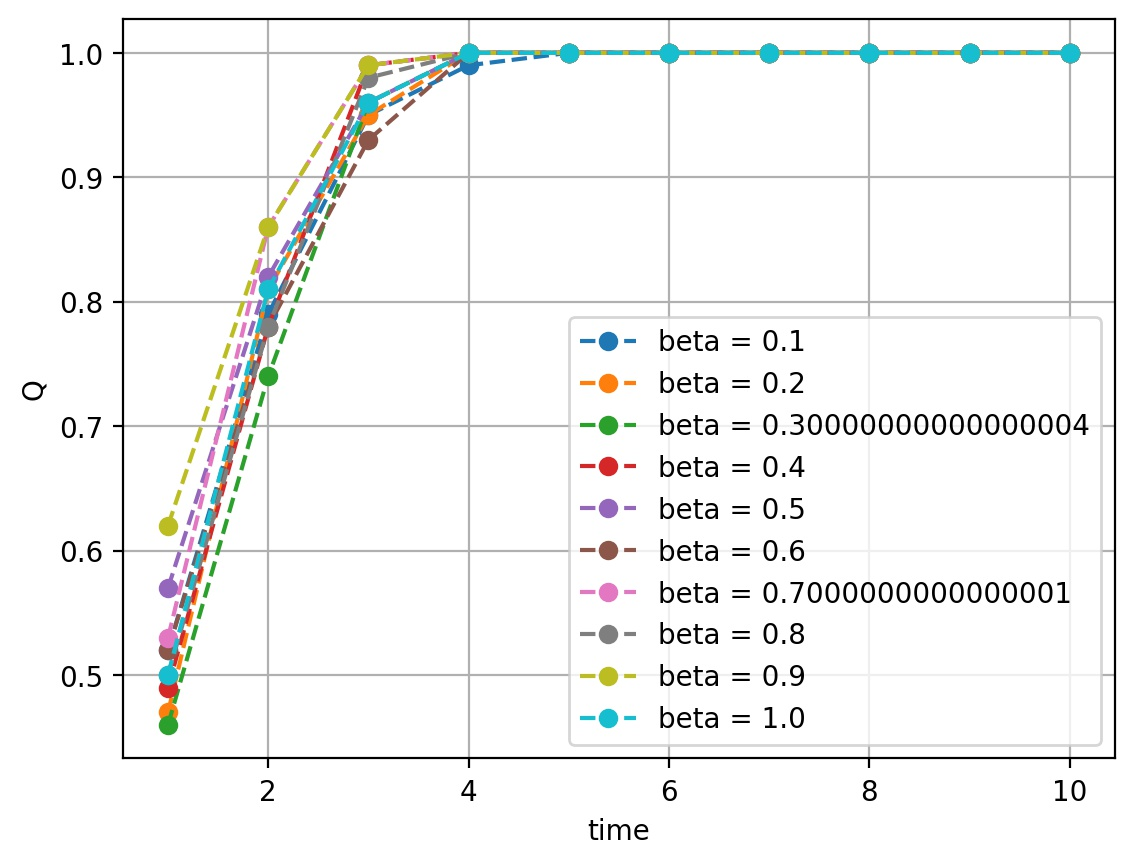
\includegraphics[width=.8\linewidth]{../results/Q_t_betas_inverted.jpg}
		\caption{The plot for Q over time for various $\beta$, with the utility matrix transposed.}
		\label{fig:Qs_inverse}
	\end{figure}
	
	\section{Section 3}
	Now we add the probability that a player revolts. The results for the previous sections are regenerated, taking this probability into account.
	Fig~\ref{fig:revolt}
	\begin{figure}[h!]
		\centering
		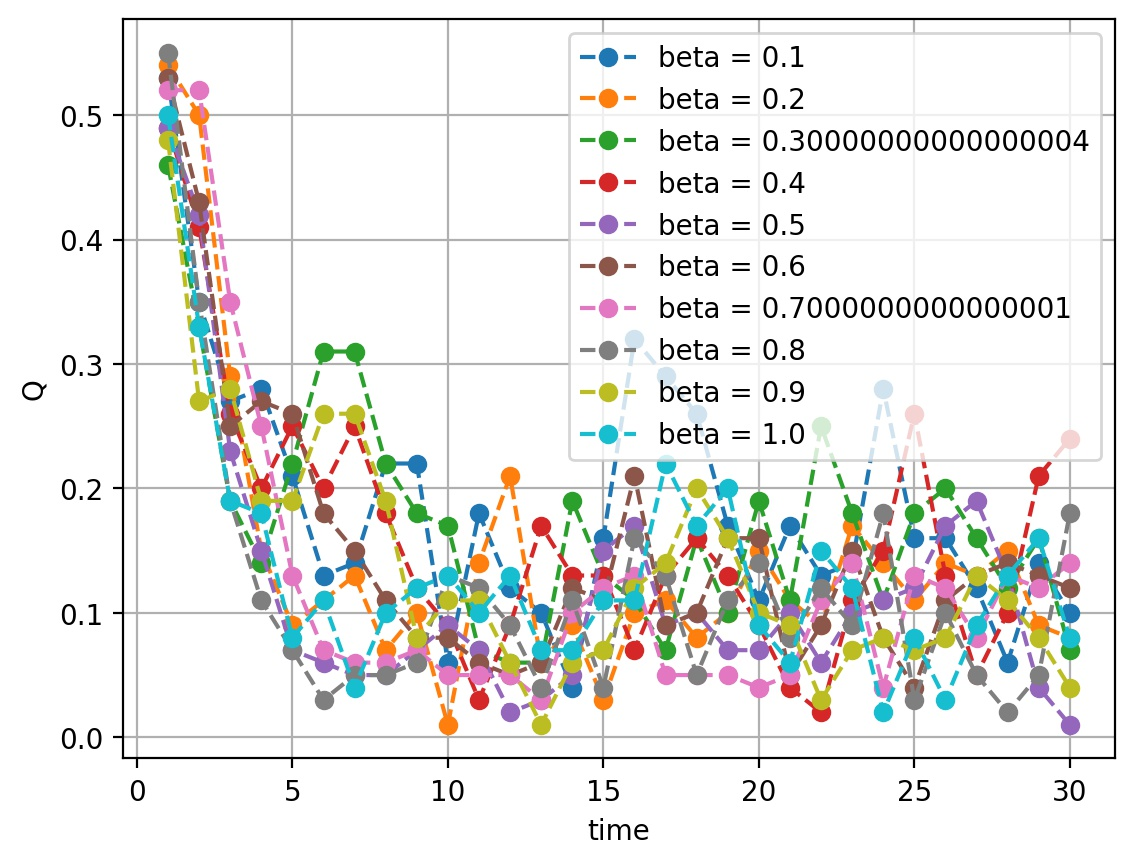
\includegraphics[width=.45\linewidth]{../results/Q_t_betas_rev_1.jpg}
		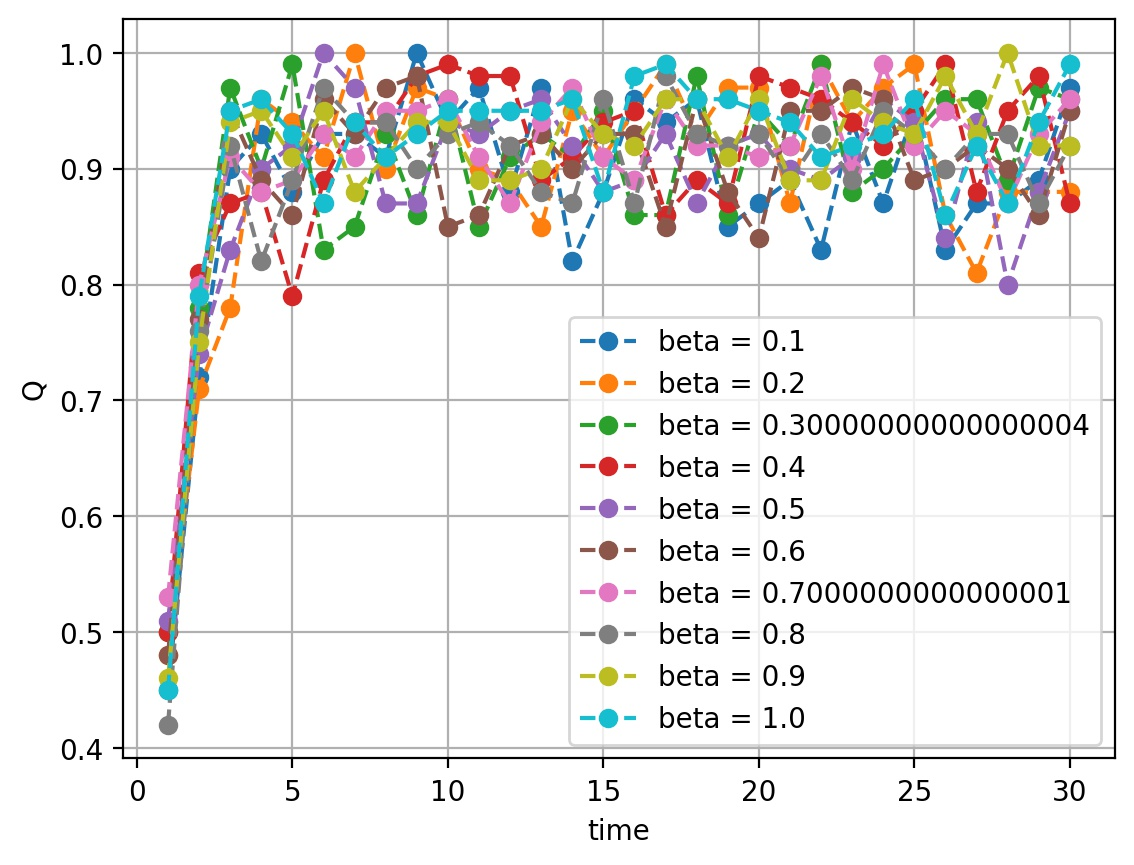
\includegraphics[width=.45\linewidth]{../results/Q_t_betas_rev_2.jpg}
		\caption{Again the equilibrium is on 0 and 1 but there are fluctuations due to the revolting of the players.}
		\label{fig:revolt}
	\end{figure}
\end{document}